\section{Cr�er un enseignement}

\begin{flushleft}
Un enseignant peut cr�er un nouvel enseignement. 
Il devient alors responsable de cet enseignement.\\
Un enseignement est caract�ris� par une section - une mati�re - une ann�e
(ex : Maitrise - Genie Logiciel - 2003)
L'enseignant doit renseigner ces trois champs pour cr�er une enseignement.
Pour �viter les cr�ations multiples de mati�res (ex :maths
math�matiques ...), on met � disposition un module une saisie des donn�es semi-automatique, c'est-�-dire que lorsque l'utilisateur saisit les
diff�rents champs, l'application essaie de compl�ter avec des noms
existants dans la base. Cela facilite ainsi la tache �
l'utilisateur.\\
De plus, une liste d�roulante est associ�e � chaque champ. Ces listes
contiennent l'ensemble des sections (si on est dans le champ section)
tri�es par ordre alphab�tique, ce qui permet encore une fois une saisie
rapide et ais�e pour l'utilisateur. 

\scalebox{0.5}{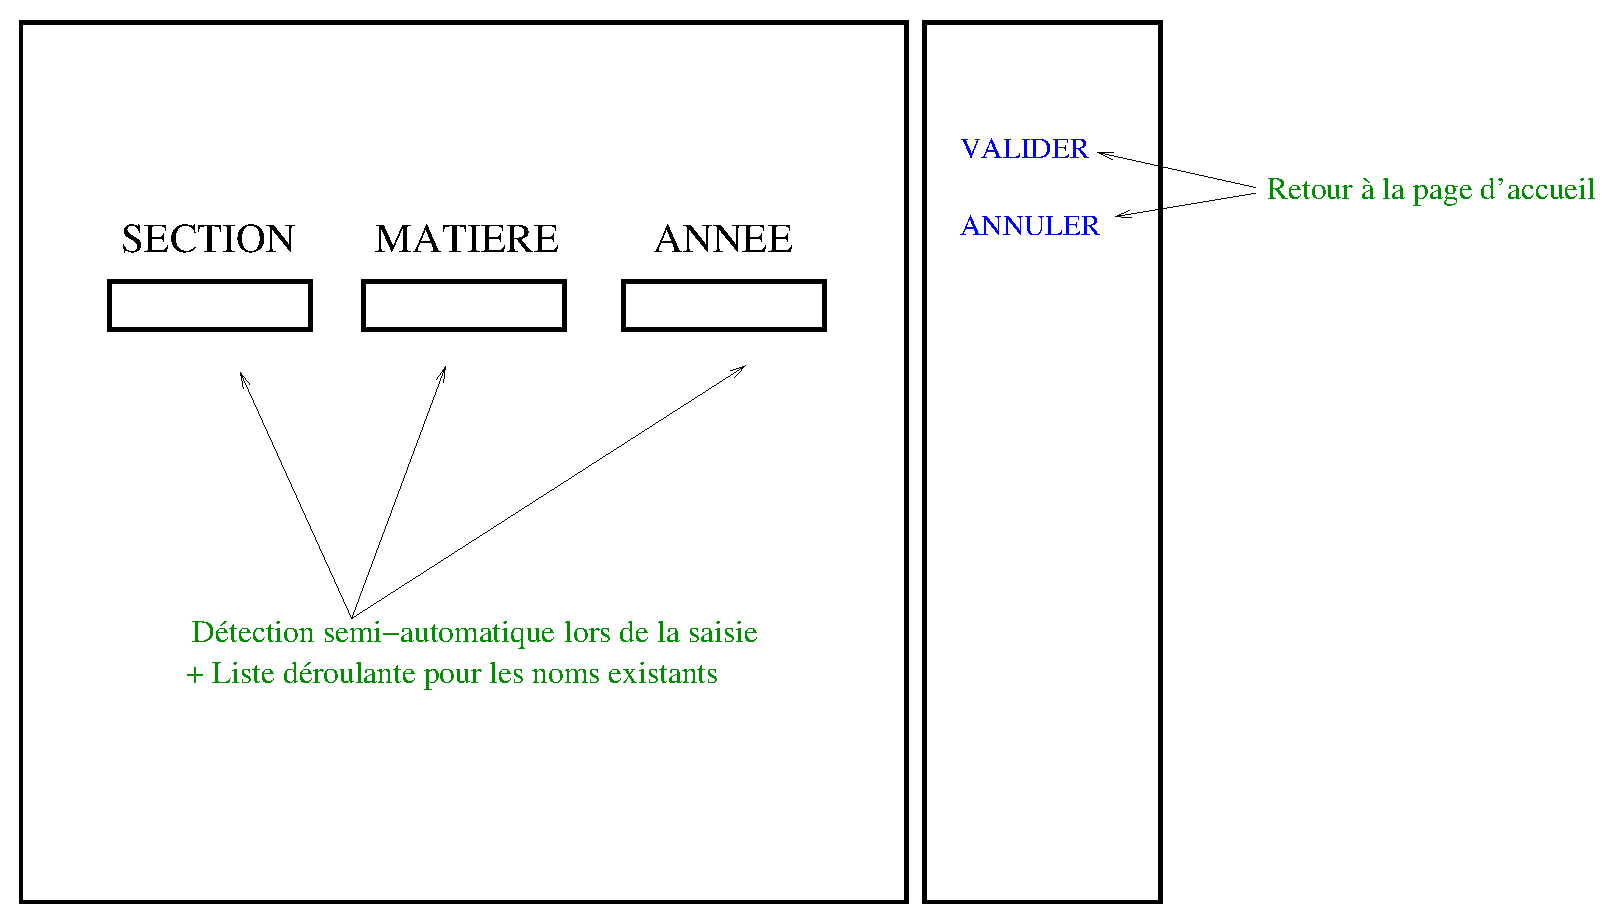
\includegraphics{../eps/enseignementMain.eps}}\\
{\it Page principale de la cr�ation d'un enseignement}
\end{flushleft}


Pour cr�er l'enseignement l'enseignant clique sur le lien "valider".
La page suivante indique l'enseignement cr�er.
\begin{flushleft}
\scalebox{0.5}{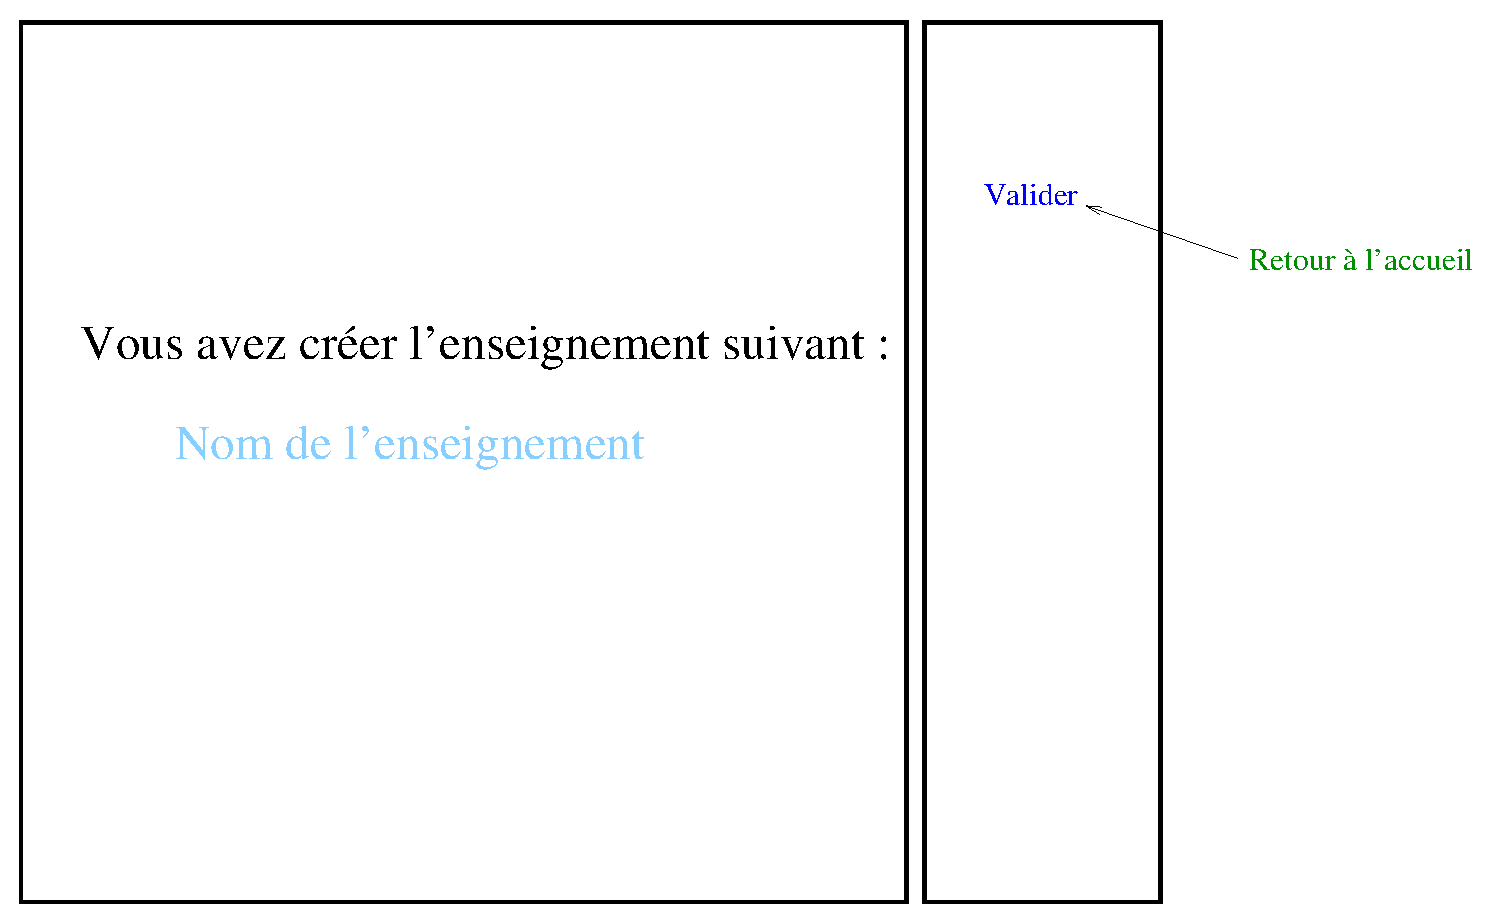
\includegraphics{../eps/enseignementOK.eps}}\\
{\it Cr�ation r�ussie}
\end{flushleft}


Si il y a eu une erreur lors de la saisie des renseignements, un message d'erreur apparait.
\begin{flushleft}
\scalebox{0.5}{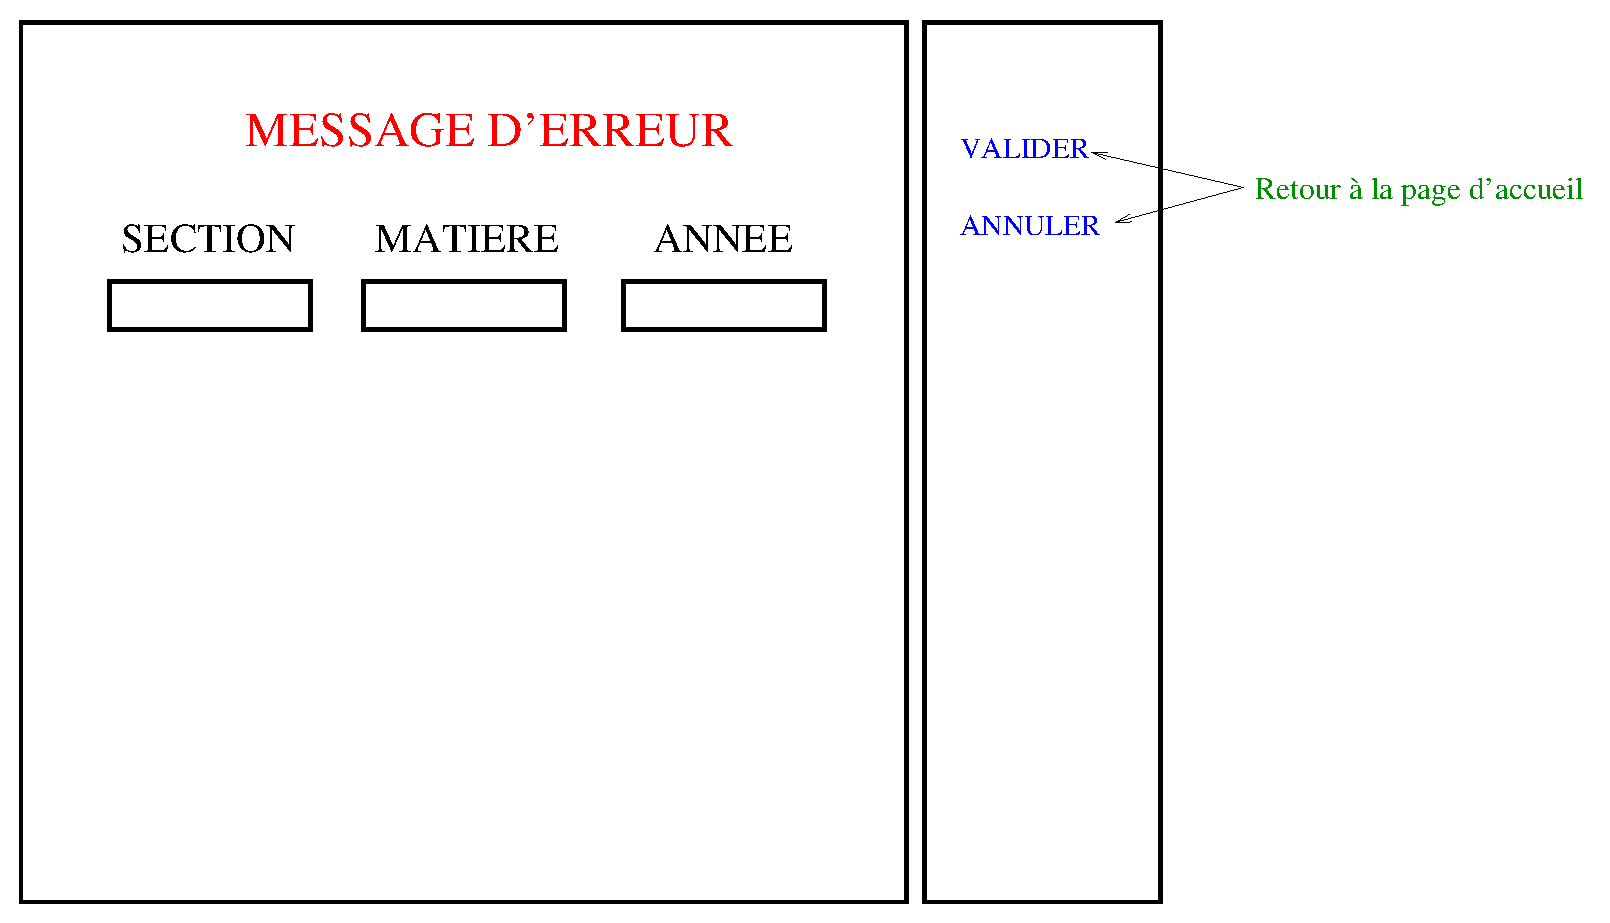
\includegraphics{../eps/enseignementNOK.eps}}\\
{\it Cr�ation �chou�e}
\end{flushleft}









